\documentclass{article}
\usepackage{graphicx}
\usepackage{subcaption}
\usepackage{geometry}
\usepackage{tikz}
\usepackage{amsmath}
\usepackage{cleveref}
\usepackage{float}
\usepackage[useregional]{datetime2}
\def\checkmark{\tikz\fill[scale=0.4](0,.35) -- (.25,0) -- (1,.7) -- (.25,.15) -- cycle;}
\usepackage[font=small,skip=0pt]{caption}
\geometry{legalpaper, margin=1in}
\title{STAT 8003 Homework 1}
\author{Zhijia Chen}
\date{\today}

\begin{document}

\begin{titlepage}
    \maketitle
\end{titlepage}

\textbf{problem 1.}

\vspace{\baselineskip}
\textit{question 1.1.}

population of interest: Time Magazine articles contributed by FZ.

population quantity of interest: the number of Time Magazine articles contributed by FZ.

sampling units: article

\vspace{\baselineskip}
\textit{question 1.2.}

The average and the variance of the number of times that the word \textbf{however} being used \textbf{per article}, the average and the variance of the number of times that the word \textbf{however} being used \textbf{per sentence}.

\vspace{\baselineskip}
\textit{question 1.3.}

\begin{table}[H]
    \centering
    \begin{minipage}[b]{.3\textwidth}
        \centering
        \begin{tabular}{| c | c | c |}
            \hline
            & {\small varibale} & {\small constant} \\
            \hline
            {\small observed}& \checkmark &  \\
            \hline
            {\small unknown} &  &  \\
            \hline
        \end{tabular}
        \captionof{table}{\textit{X\textsubscript{i}, ..., X\textsubscript{n}}}
    \end{minipage}
    \begin{minipage}[b]{.3\textwidth}
        \centering
        \begin{tabular}{| c | c | c |}
            \hline
            & {\small varibale} & {\small constant} \\
            \hline
            {\small observed}&  & \checkmark \\
            \hline
            {\small unknown} &  & \\
            \hline
            \end{tabular}
        \captionof{table}{\textit{x\textsubscript{i}, ..., x\textsubscript{n}}}
    \end{minipage}
\end{table}

\begin{table}[H]
    \centering
    \begin{minipage}[b]{.3\textwidth}
        \centering
        \begin{tabular}{| c | c | c |}
            \hline
            & {\small varibale} & {\small constant} \\
            \hline
            {\small observed}&  &  \\
            \hline
            {\small unknown} & \checkmark &  \\
            \hline
        \end{tabular}
        \captionof{table}{\textit{$\lambda$}}
    \end{minipage}
    \begin{minipage}[b]{.3\textwidth}
        \centering
        \begin{tabular}{| c | c | c |}
            \hline
            & {\small varibale} & {\small constant} \\
            \hline
            {\small observed}&  & \checkmark \\
            \hline
            {\small unknown} &  & \\
            \hline
            \end{tabular}
        \captionof{table}{\textit{n}}
    \end{minipage}
\end{table}

\vspace{\baselineskip}
\textit{question 1.4.}

$$p(X_i=x_i|\lambda) = \frac{\lambda^{x_i}e^{-\lambda}}{x_i!}$$

\vspace{\baselineskip}
\textit{question 1.5.}

\begin{enumerate}
    \item Generate a random number p that follows the uniform distribution $U(0, 1)$.
    \item Denote the cumulative distribution function(CDF) of Poission($X|\lambda$) as $cp(X)$.
    \item Find $X$ such that $cp(X)\geq p$ and $cp(X-1)<p$, then $X$ is a random variable that fits the model.
\end{enumerate}
  
\vspace{\baselineskip}
\textit{question 1.6.}
$$L(\lambda)=\prod_{i=1}^np(X_i|\lambda)=\prod_{i=1}^n\frac{\lambda^{X_i}e^{-\lambda}}{X_i!}$$

\vspace{\baselineskip}
\textit{question 1.7.}
\begin{align*}
    l(\lambda)&=log(L(\lambda))\\&=\sum_{i=1}^nlog(\frac{\lambda^{X_i}e^{-\lambda}}{X_i!})\\&=\sum_{i=1}^n(X_ilog(\lambda) - \lambda - log(X_i!))\\&= log(\lambda)\sum_{i=1}^n X_i - n\lambda - \sum_{i=1}^nlog(X_i!)
\end{align*}

\vspace{\baselineskip}
\textit{question 1.8.}
\begin{align*}
    l(\lambda)&=log(\lambda)(12+4+5+3+7+5+6) \\&- (log(12!)+log(4!)+log(5!)+log(3!)+log(7!)+log(5!)+log(6!)) \\&- 7\lambda
\end{align*}

\vspace{\baselineskip}
\textit{question 1.9.}

As shown by figure \ref{fig:1-9}, the $lambda$ value of maximum likelihood is 6.

\begin{figure}[H]
    \centering
    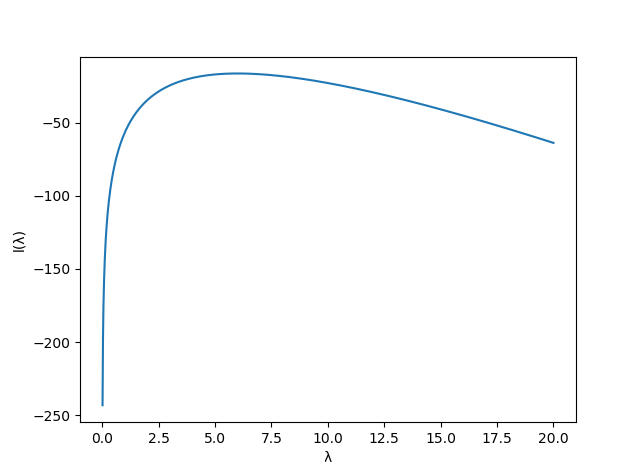
\includegraphics[width=0.5\textwidth]{1-9}
    \caption{question 1.9.}
    \label{fig:1-9}
\end{figure}

\vspace{\baselineskip}
\textit{question 1.10.}

See figure ~\ref{fig:1-10}.

\begin{figure}[H]
    \centering
        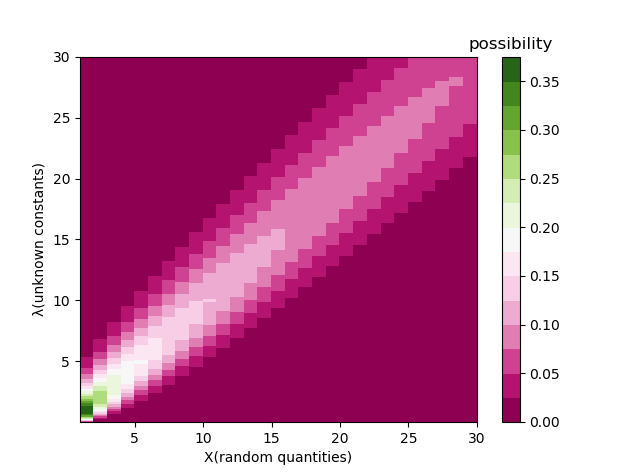
\includegraphics[width=0.5\textwidth]{1-10}
    \caption{question 1.10.}
    \label{fig:1-10}
\end{figure}

\vspace{\baselineskip}
\textbf{problem 2.}

\vspace{\baselineskip}
\textit{question 2.1.}

\begin{table}[H]
    \centering
    \begin{minipage}[b]{.3\textwidth}
        \begin{tabular}{| c | c | c |}
            \hline
            & {\small varibale} & {\small constant} \\
            \hline
            {\small observed}& \checkmark &  \\
            \hline
            {\small unknown} &  &  \\
            \hline
        \end{tabular}
        \captionof{table}{\textit{X\textsubscript{i}, ..., X\textsubscript{n}}}
    \end{minipage}
    \begin{minipage}[b]{.3\textwidth}
        \begin{tabular}{| c | c | c |}
            \hline
            & {\small varibale} & {\small constant} \\
            \hline
            {\small observed}& & \checkmark \\
            \hline
            {\small unknown} &  &  \\
            \hline
        \end{tabular}
        \captionof{table}{\textit{x\textsubscript{i}, ..., x\textsubscript{n}}}
    \end{minipage}
    \begin{minipage}[b]{.3\textwidth}
        \begin{tabular}{| c | c | c |}
            \hline
            & {\small varibale} & {\small constant} \\
            \hline
            {\small observed}& & \checkmark \\
            \hline
            {\small unknown} &  &  \\
            \hline
        \end{tabular}
        \captionof{table}{\textit{y\textsubscript{i}, ..., y\textsubscript{n}}}
    \end{minipage}
\end{table}

\begin{table}[H]
    \centering
    \begin{minipage}[b]{.3\textwidth}
        \begin{tabular}{| c | c | c |}
            \hline
            & {\small varibale} & {\small constant} \\
            \hline
            {\small observed}& &  \\
            \hline
            {\small unknown} &  & \checkmark \\
            \hline
        \end{tabular}
        \captionof{table}{\textit{$\nu$}}
    \end{minipage}
    \begin{minipage}[b]{.3\textwidth}
        \begin{tabular}{| c | c | c |}
            \hline
            & {\small varibale} & {\small constant} \\
            \hline
            {\small observed}& & \checkmark \\
            \hline
            {\small unknown} &  &  \\
            \hline
        \end{tabular}
        \captionof{table}{\textit{n}}
    \end{minipage}
\end{table}

\vspace{\baselineskip}
\textit{question 2.2.}

Normalization factor for article length. More words a person has written in an article, more likely the word \textit{however} is used, so the length of an article need to be normalized.

\vspace{\baselineskip}
\textit{question 2.3.}

A constant to fit the Poission Distribution model.

\vspace{\baselineskip}
\textit{question 2.4.}

\begin{enumerate}
    \item Generate a random number p that follows the uniform distribution $U(0, 1)$.
    \item Denote the cumulative distribution function(CDF) of $Poission(x|\nu, \frac{y_i}{1000})$ as $cp(x)$.
    \item Find $X$ such that $cp(x)\geq p$ and $cp(x-1)<p$, then $x$ is a random variable that fits the model.
\end{enumerate}

\vspace{\baselineskip}
\textit{question 2.5.}

$$L(y_i,\nu,1000)=p(X_i|y_i,\nu,1000)=\frac{{(\frac{\nu y_i}{1000})}^{X_i}e^{-(\frac{\nu y_i}{1000})}}{X_i!}$$

\vspace{\baselineskip}
\textit{question 2.6.}

$$L(\nu)=\prod_{i=1}^np(X_i|y_i,\nu,1000)=\prod_{i=1}^n\frac{{(\frac{\nu y_i}{1000})}^{X_i}e^{-(\frac{\nu y_i}{1000})}}{X_i!}$$

\vspace{\baselineskip}
\textit{question 2.7.}

$$l(\nu)=log(L(\nu))=\sum_{i=1}^nlog(\frac{{(\frac{\nu y_i}{1000})}^{X_i}e^{-(\frac{\nu y_i}{1000})}}{X_i!})=
\sum_{i=1}^n(X_ilog(\frac{\nu y_i}{1000}) - \frac{\nu y_i}{1000} - log(X_i!))$$

\vspace{\baselineskip}
\textit{question 2.8.}

25, 8, 16, 10, 12

\vspace{\baselineskip}
\textit{question 2.9.}

\begin{align*}
    l(\nu)=
    &(191log(1.73\nu) - 1.73\nu - log(191!)) +\\
    &(93log(0.947\nu) - 0.947\nu - log(93!)) +\\
    &(182log(1.83\nu) - 1.83\nu - log(182!)) +\\
    &(104log(1.21\nu) - 1.21\nu - log(104!)) +\\
    &(96log(1.1\nu) - 1.1\nu - log(96!))   
\end{align*}




\vspace{\baselineskip}
\textit{question 2.10.}

As shown by figure ~\ref{fig:2-10}, the $\nu $ value of maximum likelihood is 9.53.

\begin{figure}[H]
    \centering
    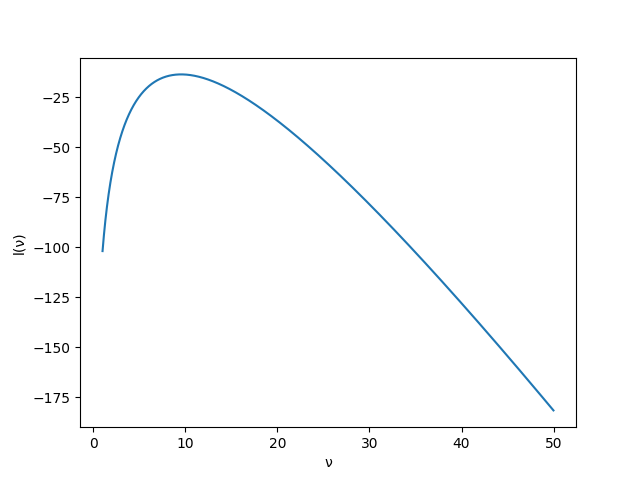
\includegraphics[width=0.5\textwidth]{2-10}
    \caption{question 2.10.}
    \label{fig:2-10}
\end{figure}

\vspace{\baselineskip}
\textit{question 2.11.}

See figure ~\ref{fig:2-11}.

\begin{figure}[H]
    \centering
        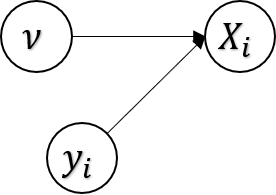
\includegraphics[width=0.5\textwidth]{2-11}
    \caption{question 2.11.}
    \label{fig:2-11}
\end{figure}


\vspace{\baselineskip}
\textbf{problem 3.}

\vspace{\baselineskip}
\textit{question 3.1.}

\begin{table}[H]
    \centering
    \begin{minipage}[b]{.3\textwidth}
        \begin{tabular}{| c | c | c |}
            \hline
            & {\small varibale} & {\small constant} \\
            \hline
            {\small observed}& \checkmark &  \\
            \hline
            {\small unknown} &  &  \\
            \hline
        \end{tabular}
        \captionof{table}{\textit{X\textsubscript{i}, ..., X\textsubscript{n}}}
    \end{minipage}
    \begin{minipage}[b]{.3\textwidth}
        \begin{tabular}{| c | c | c |}
            \hline
            & {\small varibale} & {\small constant} \\
            \hline
            {\small observed}& & \checkmark \\
            \hline
            {\small unknown} &  &  \\
            \hline
        \end{tabular}
        \captionof{table}{\textit{x\textsubscript{i}, ..., x\textsubscript{n}}}
    \end{minipage}
    \begin{minipage}[b]{.3\textwidth}
        \begin{tabular}{| c | c | c |}
            \hline
            & {\small varibale} & {\small constant} \\
            \hline
            {\small observed}& \checkmark & \\
            \hline
            {\small unknown} &  &  \\
            \hline
        \end{tabular}
        \captionof{table}{\textit{Z\textsubscript{i}, ..., Z\textsubscript{n}}}
    \end{minipage}
\end{table}

\begin{table}[H]
    \centering
    \begin{minipage}[b]{.3\textwidth}
        \begin{tabular}{| c | c | c |}
            \hline
            & {\small varibale} & {\small constant} \\
            \hline
            {\small observed}& & \checkmark \\
            \hline
            {\small unknown} &  &  \\
            \hline
        \end{tabular}
        \captionof{table}{\textit{z\textsubscript{i}, ..., z\textsubscript{n}}}
    \end{minipage}
    \begin{minipage}[b]{.3\textwidth}
        \begin{tabular}{| c | c | c |}
            \hline
            & {\small varibale} & {\small constant} \\
            \hline
            {\small observed}& & \\
            \hline
            {\small unknown} &  & \checkmark \\
            \hline
        \end{tabular}
        \captionof{table}{\textit{$\pi$}}
    \end{minipage}
    \begin{minipage}[b]{.3\textwidth}
        \begin{tabular}{| c | c | c |}
            \hline
            & {\small varibale} & {\small constant} \\
            \hline
            {\small observed}& & \\
            \hline
            {\small unknown} &  & \checkmark \\
            \hline
        \end{tabular}
        \captionof{table}{\textit{${\lambda}_{Politics}$}}
    \end{minipage}
\end{table}

\begin{table}[H]
    \centering
    \begin{minipage}[b]{.3\textwidth}
        \begin{tabular}{| c | c | c |}
            \hline
            & {\small varibale} & {\small constant} \\
            \hline
            {\small observed}& & \\
            \hline
            {\small unknown} &  & \checkmark \\
            \hline
        \end{tabular}
        \captionof{table}{\textit{${\theta}_{Other}$}}
    \end{minipage}
    \begin{minipage}[b]{.3\textwidth}
        \begin{tabular}{| c | c | c |}
            \hline
            & {\small varibale} & {\small constant} \\
            \hline
            {\small observed}& & \checkmark \\
            \hline
            {\small unknown} &  & \\
            \hline
        \end{tabular}
        \captionof{table}{\textit{n}}
    \end{minipage}
\end{table}

\vspace{\baselineskip}
\textit{question 3.2.}

\begin{enumerate}
    \item Generate a random number z ~ $Bernoulli(z, \pi)$.
    \item Generate a random number p ~ $U(0, 1)$.
    \item Denote the CDF of $Poission(x|\nu, \frac{y_i}{1000})$ as $cp1(x)$, and the CDF of $Binomial(x|1000, \theta_{other})$ as $cp0(x)$.
    \item If z = 1, find $x$ such that $cp1(x)\geq p$ and $cp1(x-1)<p$, otherwise find $x$ such that $cp0(x)\geq p$ and $cp0(x-1)<p$.
\end{enumerate}

\vspace{\baselineskip}
\textit{question 3.3.}

See figure \ref{fig:3-3}.

\begin{figure}[H]
    \centering
    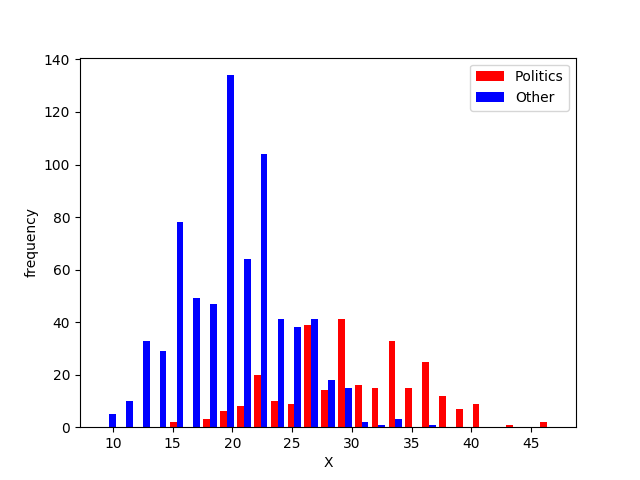
\includegraphics[width=0.5\textwidth]{3-3}
    \caption{question 3.3.}
    \label{fig:3-3}
\end{figure}

\vspace{\baselineskip}
\textit{question 3.4.}

\begin{align*}
    L_i(\lambda_{Politics}, \theta_{Other})&=p(X_i=x_i|\lambda_{Politics}, \theta_{Other})\\&=p(Z_i=1)Poission(x_i|\lambda_{Politics})+p(Z_i=0)Binomial(x_i|1000,\theta_{Other})\\&=\pi\frac{\lambda_{Politics}^{x_i}e^{-\lambda_{Politics}}}{x_i!}+(1-\pi){1000\choose x_i}{(1-\theta_{Other})}^{x_i}\theta_{Other}^{1000-x_i} 
\end{align*}


\vspace{\baselineskip}
\textit{question 3.5.}

$$L(\lambda_{Politics}, \theta_{Other})=\prod_{i=1}^n\left(\pi\frac{\lambda_{Politics}^{x_i}e^{-\lambda_{Politics}}}{x_i!}+(1-\pi){1000\choose x_i}{(1-\theta_{Other})}^{x_i}\theta_{Other}^{1000-x_i}\right)$$

\vspace{\baselineskip}
\textit{question 3.6.}

$$l(\lambda_{Politics}, \theta_{Other})=\sum_{i=1}^nlog\left(\pi\frac{\lambda_{Politics}^{x_i}e^{-\lambda_{Politics}}}{x_i!}+(1-\pi){1000\choose x_i}{(1-\theta_{Other})}^{x_i}\theta_{Other}^{1000-x_i}\right)$$

\vspace{\baselineskip}
\textit{question 3.7.}

\begin{align*}
    l(\lambda_{Politics}, \theta_{Other})&=\left(\pi\frac{\lambda_{Politics}^{12}e^{-\lambda_{Politics}}}{12!}+(1-\pi){1000\choose 12}{(1-\theta_{Other})}^{12}\theta_{Other}^{1000-12}\right)\\&+\left(\pi\frac{\lambda_{Politics}^{4}e^{-\lambda_{Politics}}}{4!}+(1-\pi){1000\choose 4}{(1-\theta_{Other})}^{4}\theta_{Other}^{1000-4}\right)\\&+\left(\pi\frac{\lambda_{Politics}^{8}e^{-\lambda_{Politics}}}{8!}+(1-\pi){1000\choose 8}{(1-\theta_{Other})}^{8}\theta_{Other}^{1000-8}\right)\\&+2\left(\pi\frac{\lambda_{Politics}^{3}e^{-\lambda_{Politics}}}{3!}+(1-\pi){1000\choose 3}{(1-\theta_{Other})}^{3}\theta_{Other}^{1000-3}\right)\\&+\left(\pi\frac{\lambda_{Politics}^{1}e^{-\lambda_{Politics}}}{1!}+(1-\pi){1000\choose 1}{(1-\theta_{Other})}^{1}\theta_{Other}^{1000-1}\right)\\&+\left(\pi\frac{\lambda_{Politics}^{9}e^{-\lambda_{Politics}}}{9!}+(1-\pi{1000\choose 9}{(1-\theta_{Other})}^{9}\theta_{Other}^{1000-9}\right)
\end{align*}



\vspace{\baselineskip}
\textit{question 3.8.}

See figure ~\ref{fig:3-8}.

\begin{figure}[H]
    \centering
        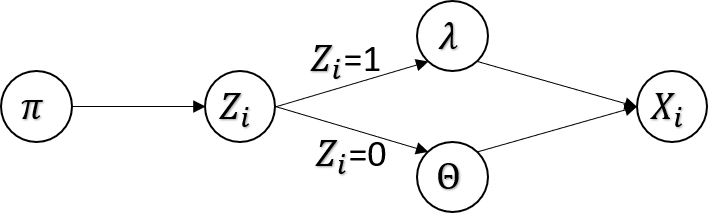
\includegraphics[width=0.5\textwidth]{3-8}
    \caption{question 3.8.}
    \label{fig:3-8}
\end{figure}


\vspace{\baselineskip}
\textbf{problem 4.}

\vspace{\baselineskip}
\textit{question 4.1.}


\begin{table}[H]
    \centering
    \begin{minipage}[b]{.3\textwidth}
        \begin{tabular}{| c | c | c |}
            \hline
            & {\small varibale} & {\small constant} \\
            \hline
            {\small observed}& \checkmark & \\
            \hline
            {\small unknown} &  &  \\
            \hline
        \end{tabular}
        \captionof{table}{\textit{X\textsubscript{i}, ..., X\textsubscript{n}}}
    \end{minipage}
    \begin{minipage}[b]{.3\textwidth}
        \begin{tabular}{| c | c | c |}
            \hline
            & {\small varibale} & {\small constant} \\
            \hline
            {\small observed}& & \checkmark \\
            \hline
            {\small unknown} &  & \\
            \hline
        \end{tabular}
        \captionof{table}{\textit{x\textsubscript{i}, ..., x\textsubscript{n}}}
    \end{minipage}
    \begin{minipage}[b]{.3\textwidth}
        \begin{tabular}{| c | c | c |}
            \hline
            & {\small varibale} & {\small constant} \\
            \hline
            {\small observed}& & \\
            \hline
            {\small unknown} & \checkmark & \\
            \hline
        \end{tabular}
        \captionof{table}{\textit{$\Lambda$}}
    \end{minipage}
\end{table}

\begin{table}[H]
    \centering
    \begin{minipage}[b]{.3\textwidth}
        \begin{tabular}{| c | c | c |}
            \hline
            & {\small varibale} & {\small constant} \\
            \hline
            {\small observed}&  & \\
            \hline
            {\small unknown} &  & \checkmark\\
            \hline
        \end{tabular}
        \captionof{table}{\textit{$\lambda$\textsubscript{i}, ..., $\lambda$\textsubscript{n}}}
    \end{minipage}
    \begin{minipage}[b]{.3\textwidth}
        \begin{tabular}{| c | c | c |}
            \hline
            & {\small varibale} & {\small constant} \\
            \hline
            {\small observed}& & \checkmark \\
            \hline
            {\small unknown} &  & \\
            \hline
        \end{tabular}
        \captionof{table}{\textit{$\alpha$}}
    \end{minipage}
    \begin{minipage}[b]{.3\textwidth}
        \begin{tabular}{| c | c | c |}
            \hline
            & {\small varibale} & {\small constant} \\
            \hline
            {\small observed}& & \\
            \hline
            {\small unknown} &  & \checkmark \\
            \hline
        \end{tabular}
        \captionof{table}{\textit{$\theta$}}
    \end{minipage}
\end{table}

\begin{table}[H]
    \centering
    \begin{minipage}[b]{.3\textwidth}
        \begin{tabular}{| c | c | c |}
            \hline
            & {\small varibale} & {\small constant} \\
            \hline
            {\small observed}&  & \checkmark \\
            \hline
            {\small unknown} &  & \\
            \hline
        \end{tabular}
        \captionof{table}{\textit{n}}
    \end{minipage}
\end{table}

\vspace{\baselineskip}
\textit{question 4.2.}

\begin{enumerate}
    \item Generate a random number $\lambda ~ Gamma(\lambda, \alpha, \theta)$
    \item Generate a random number $p ~ U(0, 1)$.
    \item Denote the CDF of $Poission(x|\lambda)$ as $cp(x$.
    \item Find $x$ such that $cp(x)\geq p$ and $cp(x-1)<p$.
\end{enumerate}

\vspace{\baselineskip}
\textit{question 4.3.}

Mean: 9.931

Variance: 21.138

\vspace{\baselineskip}
\textit{question 4.4.}

Mean: 9.856

Variance: 9.461

The mean is similar, while the variance is much smaller in this case.

\vspace{\baselineskip}
\textit{question 4.5.}
\begin{align*}
    L_i(\alpha, \theta)&=\int_0^\infty Poission(x_i|\lambda_i)Gamma(\lambda_i|\alpha, \theta)dx\\&=\int_0^\infty\left(\frac{\lambda_i^{x_i}e^{-\lambda_i}}{x_i!}\frac{\theta^\alpha}{\Gamma(\alpha)}\lambda_i^{\alpha-1}e^{-\theta\lambda_i}\right)d\lambda_i
\end{align*}

\vspace{\baselineskip}
\textit{question 4.6.}

$$l(\alpha, \theta)=\sum_i^n\left(log\left(\int_0^\infty\left(\frac{\lambda_i^{x_i}e^{-\lambda_i}}{x_i!}\frac{\theta^\alpha}{\Gamma(\alpha)}\lambda_i^{\alpha-1}e^{-\theta\lambda_i}\right)d\lambda_i\right)\right)$$

\vspace{\baselineskip}
\textit{question 4.7.}

\begin{align*}
    l(\alpha, \theta)&=log\left(\int_0^\infty\left(\frac{\lambda_i^{64}e^{-\lambda}}{64!}\frac{\theta^\alpha}{\Gamma(\alpha)}\lambda^{\alpha-1}e^{-\theta\lambda}\right)d\lambda\right)\\&+
    log\left(\int_0^\infty\left(\frac{\lambda_i^{61}e^{-\lambda}}{61!}\frac{\theta^\alpha}{\Gamma(\alpha)}\lambda^{\alpha-1}e^{-\theta\lambda}\right)d\lambda\right)\\&+
    log\left(\int_0^\infty\left(\frac{\lambda_i^{89}e^{-\lambda}}{89!}\frac{\theta^\alpha}{\Gamma(\alpha)}\lambda^{\alpha-1}e^{-\theta\lambda}\right)d\lambda\right)\\&+
    log\left(\int_0^\infty\left(\frac{\lambda_i^{55}e^{-\lambda}}{55!}\frac{\theta^\alpha}{\Gamma(\alpha)}\lambda^{\alpha-1}e^{-\theta\lambda}\right)d\lambda\right)\\&+
    log\left(\int_0^\infty\left(\frac{\lambda_i^{57}e^{-\lambda}}{57!}\frac{\theta^\alpha}{\Gamma(\alpha)}\lambda^{\alpha-1}e^{-\theta\lambda}\right)d\lambda\right)\\&+
    log\left(\int_0^\infty\left(\frac{\lambda_i^{76}e^{-\lambda}}{76!}\frac{\theta^\alpha}{\Gamma(\alpha)}\lambda^{\alpha-1}e^{-\theta\lambda}\right)d\lambda\right)\\&+
    log\left(\int_0^\infty\left(\frac{\lambda_i^{74}e^{-\lambda}}{74!}\frac{\theta^\alpha}{\Gamma(\alpha)}\lambda^{\alpha-1}e^{-\theta\lambda}\right)d\lambda\right)\\&+
    log\left(\int_0^\infty\left(\frac{\lambda_i^{55}e^{-\lambda}}{55!}\frac{\theta^\alpha}{\Gamma(\alpha)}\lambda^{\alpha-1}e^{-\theta\lambda}\right)d\lambda\right)
\end{align*}



\vspace{\baselineskip}
\textit{question 4.8.}

See figure ~\ref{fig:4-8}.

\begin{figure}[H]
    \centering
        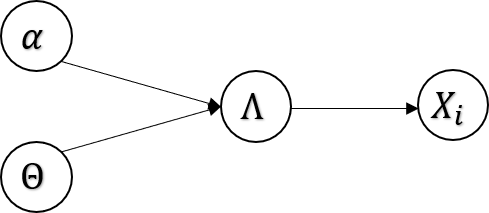
\includegraphics[width=0.5\textwidth]{4-8}
    \caption{question 4.8.}
    \label{fig:4-8}
\end{figure}


\end{document}

